 \begin{frame}
  \frametitle{Architecture Altarica}
  \center
  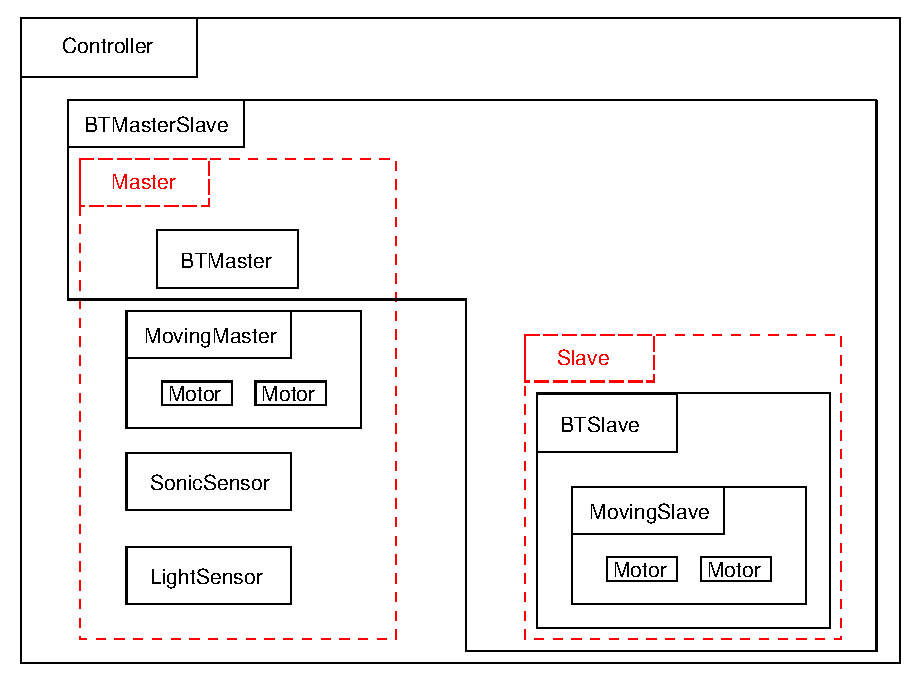
\includegraphics[height=7cm]{ARmodel.eps}

 \end{frame}
 
 
 \begin{frame}
  \frametitle{N\oe{}ud LightSensor}

  \begin{block}{2ème version du noeud}
   \verbatiminput{../src/altarica/alt/LightSensor.alt}
  \end{block}
  
  \begin{block}{}
   \begin{itemize}
    \item Au début, variable d'état
	  \uncover<2->{
    \item Mais l'environnement est incontrôlable}
	  \uncover<3->{
    \item donc utilisation d'une variable de flux}
	  \uncover<4->{
    \item trois seuils de couleur à détecter}
   \end{itemize}
  \end{block}

 \end{frame}
 
  \begin{frame}
  \frametitle{N\oe{}ud Moving master}

    \begin{block}{}
    \verbatiminput{../src/altarica/alt/MovingMaster.alt}
    \end{block}

  \end{frame}

  \begin{frame}
   \frametitle{N\oe{}ud Controller (1/12)}
   
    \verbatiminput{../src/altarica/alt/Controller1.alt}   
  \end{frame}

  \begin{frame}
   \frametitle{N\oe{}ud Controller (2/12)}
   
    \verbatiminput{../src/altarica/alt/Controller2.alt}
   
  \end{frame}
  \begin{frame}
   \frametitle{N\oe{}ud Controller (3/12)}
   
    \verbatiminput{../src/altarica/alt/Controller3.alt}
   
  \end{frame}
  \begin{frame}
   \frametitle{N\oe{}ud Controller (4/12)}
   
    \verbatiminput{../src/altarica/alt/Controller4.alt}
   
  \end{frame}
  \begin{frame}
   \frametitle{N\oe{}ud Controller (5/12)}
   
    \verbatiminput{../src/altarica/alt/Controller5.alt}
   
  \end{frame}
  \begin{frame}
   \frametitle{N\oe{}ud Controller (6/12)}
   
    \verbatiminput{../src/altarica/alt/Controller6.alt}
   
  \end{frame}
  \begin{frame}
   \frametitle{N\oe{}ud Controller (7/12)}
   
    \verbatiminput{../src/altarica/alt/Controller7.alt}
   
  \end{frame}
  \begin{frame}
   \frametitle{N\oe{}ud Controller (8/12)}
   
    \verbatiminput{../src/altarica/alt/Controller8.alt}
   
  \end{frame}
  \begin{frame}
   \frametitle{N\oe{}ud Controller (9/12)}
   
    \verbatiminput{../src/altarica/alt/Controller9.alt}
   
  \end{frame}
  \begin{frame}
   \frametitle{N\oe{}ud Controller (10/12)}
   
    \verbatiminput{../src/altarica/alt/Controller10.alt}
   
  \end{frame}
  \begin{frame}
   \frametitle{N\oe{}ud Controller (11/12)}
   
    \verbatiminput{../src/altarica/alt/Controller11.alt}
   
  \end{frame}
  \begin{frame}
   \frametitle{N\oe{}ud Controller (12/12)}
   
    \verbatiminput{../src/altarica/alt/Controller12.alt}
   
  \end{frame}

  \begin{frame}
   \frametitle{Vérification du n\oe{}ud Controller}
   
    \verbatiminput{../src/altarica/acheck/Controller.acheck}
   
  \end{frame}

  \begin{frame}
   \frametitle{Résultats}
   
   \verbatiminput{../src/altarica/Controller.prop}
   \verbatiminput{../src/altarica/Controller.res}
   
  \end{frame}

  \begin{frame}
   \frametitle{Difficultés}
   
  \begin{block}{Simulation avec \emph{arc}}
   \begin{itemize}
    \item Problème : Possibilité de tirer des transitions non voulues
    \item<2-> Cause : Événements non capturés car non utilisés
   \end{itemize}
  \end{block}
   
  \end{frame}

